% -----------------------------------------------
% Template for SMC 2020
% adapted from previous SMC paper templates
% -----------------------------------------------

\documentclass[dvipsnames, pdftex]{article}
\usepackage{tikz}
% \tikzset{>=latex}
% \tikzstyle{block} = [draw,minimum size=0.5cm]
% \usetikzlibrary{math,arrows,positioning,shapes.geometric, decorations.markings}

\usepackage{smc2020}
\usepackage{times}
\usepackage{ifpdf}
\usepackage[english]{babel}
\usepackage{cite}
\usepackage{multirow}
\usepackage[]{algorithm2e, setspace}
\usepackage{textcomp}
%%%%%%%%%%%%%%%%%%%%%%%% Some useful packages %%%%%%%%%%%%%%%%%%%%%%%%%%%%%%%
%%%%%%%%%%%%%%%%%%%%%%%% See related documentation %%%%%%%%%%%%%%%%%%%%%%%%%%
\usepackage{amsmath} % popular packages from Am. Math. Soc. Please use the 
\usepackage{amssymb}
\usepackage{cases}
% related math environments (split, subequation, cases,
%\usepackage{amsfonts}% multline, etc.)
%\usepackage{bm}      % Bold Math package, defines the command \bf{}
%\usepackage{paralist}% extended list environments
%%subfig.sty is the modern replacement for subfigure.sty. However, subfig.sty 
%%requires and automatically loads caption.sty which overrides class handling 
%%of captions. To prevent this problem, preload caption.sty with caption=false 
%\usepackage[caption=false]{caption}
%\usepackage[font=footnotesize]{subfig}


%user defined variables
\def\papertitle{Real-time Implementation of a Physical Model of the Tromba Marina} %using Finite-Difference Schemes}
\def\firstauthor{Silvin Willemsen}
\def\secondauthor{Stefan Bilbao}
\def\thirdauthor{Michele Ducceschi}
\def\fourthauthor{Stefania Serafin}
% \def\firstauthor{Silvin Willemsen, Stefania Serafin}
% \def\secondauthor{Stefan Bilbao and Michele Ducceschi}

% adds the automatic
% Saves a lot of output space in PDF... after conversion with the distiller
% Delete if you cannot get PS fonts working on your system.

% pdf-tex settings: detect automatically if run by latex or pdflatex
\newif\ifpdf
\ifx\pdfoutput\relax
\else
   \ifcase\pdfoutput
      \pdffalse
   \else
      \pdftrue
\fi

\ifpdf % compiling with pdflatex
  \usepackage[pdftex,
    pdftitle={\papertitle},
    pdfauthor={\firstauthor, \secondauthor, \thirdauthor, \fourthauthor},
    bookmarksnumbered, % use section numbers with bookmarks
    pdfstartview=XYZ % start with zoom=100% instead of full screen; 
                     % especially useful if working with a big screen :-)
   ]{hyperref}
  %\pdfcompresslevel=9

  \usepackage{graphicx}
  % declare the path(s) where your graphic files are and their extensions so 
  %you won't have to specify these with every instance of \includegraphics
  \graphicspath{{./SMC 2020 paper template LaTeX/}}
  \DeclareGraphicsExtensions{.pdf,.jpeg,.png, .eps}

  \usepackage[figure,table]{hypcap}

\else % compiling with latex
  \usepackage[dvips,
    bookmarksnumbered, % use section numbers with bookmarks
    pdfstartview=XYZ % start with zoom=100% instead of full screen
  ]{hyperref}  % hyperrefs are active in the pdf file after conversion

  \usepackage[dvips]{epsfig,graphicx}
  % declare the path(s) where your graphic files are and their extensions so 
  %you won't have to specify these with every instance of \includegraphics
  \graphicspath{{./SMC 2020 paper template LaTeX/}}
  \DeclareGraphicsExtensions{.eps}

  \usepackage[figure,table]{hypcap}
\fi

%setup the hyperref package - make the links black without a surrounding frame
\hypersetup{
    colorlinks,%
    citecolor=black,%
    filecolor=black,%
    linkcolor=black,%
    urlcolor=black
}


% Title.
% ------
\title{\papertitle}

% Authors
% Please note that submissions are NOT anonymous, therefore 
% authors' names have to be VISIBLE in your manuscript. 
%
% Single address
% To use with only one author or several with the same address
% ---------------
%\oneauthor
%   {\firstauthor} {Affiliation1 \\ %
%     {\tt \href{mailto:author1@smcnetwork.org}{author1@smcnetwork.org}}}

%Two addresses
%--------------
\twoauthors
  {\firstauthor{ and }\fourthauthor} {Multisensory Experience Lab, CREATE \\ Aalborg University Copenhagen \\
    {\tt \href{mailto:sil@create.aau.dk}{\{sil, sts\}@create.aau.dk}}}
  {\secondauthor{ and }\thirdauthor} {Acoustics and Audio Group \\ University of Edinburgh \\ %
    {\tt {\{s.bilbao, michele.ducceschi\}@ed.ac.uk}}}

% Three addresses
% --------------
%  \threeauthors
%   {\firstauthor} {Affiliation1 \\ %
%      {\tt \href{mailto:author1@smcnetwork.org}{author1@smcnetwork.org}}}
%   {\secondauthor} {Affiliation2 \\ %
%      {\tt \href{mailto:author2@smcnetwork.org}{author2@smcnetwork.org}}}
%   {\thirdauthor} { Affiliation3 \\ %
%      {\tt \href{mailto:author3@smcnetwork.org}{author3@smcnetwork.org}}}
% \fourauthors
%   {\firstauthor} {Multisensory Experience Lab, CREATE \\ Aalborg University Copenhagen \\ %
%      {\tt \href{mailto:sil@create.aau.dk}{sil@create.aau.dk}}}
%   {\secondauthor} {Acoustics and Audio Group \\ University of Edinburgh \\ %
%      {\tt \href{mailto:s.bilbao@ed.ac.uk}{s.bilbao@ed.ac.uk}}}
%     {\thirdauthor} {Acoustics and Audio Group \\ University of Edinburgh \\ %
%      {\tt \href{mailto:michele.ducceschi@ed.ac.uk}{michele.ducceschi@ed.ac.uk}}}
%   {\fourthauthor} {Multisensory Experience Lab, CREATE \\ Aalborg University Copenhagen \\ %
%      {\tt \href{mailto:sts@create.aau.dk}{sts@create.aau.dk}}}

% ***************************************** the document starts here ***************
\usepackage{xcolor}
\def\SBcomment[#1]{\textcolor{Red}{#1}}
\def\SWcomment[#1]{\textcolor{Bittersweet}{#1}}
\def\MDcomment[#1]{\textcolor{Blue}{#1}}
\def\SScomment[#1]{\textcolor{OliveGreen}{#1}}

\begin{document}
%
\capstartfalse
\maketitle
\capstarttrue
%
\begin{abstract}
You can place comments in colour if you want :) Like \SBcomment[this (Stefan)], \MDcomment[this (Michele)] or \SScomment[this (Stefania)].
\end{abstract}
%

\section{Introduction}\label{sec:introduction}
The tromba marina (see Figure 
 \ref{fig:tromba}) is a medieval monochord bowed instrument with a long quasi-trapezoidal body and a uniquely fashioned bridge (often called a shoe, because of its shape – see Figure \ref{fig:bridge}). 
 The name of the instrument derives from the fact that {\em tromba} means {\em trumpet} in Italian. As a matter of fact,
 a foot of the bridge is free to rattle against the soundboard of the instrument in sympathy with the vibrating string. 
 This unusual bridge creates a trumpet-like sound.
 The frequency produced by the instrument is varied by placing the side of the knuckle of the non-dominant hand, lightly, at specific nodal points on the string, in order to select various harmonics of the open string. The dominant hand controls the bow, which is drawn across the string above the non-dominant hand \cite{munrow1976instruments}.
 
 
 
  
   \begin{figure}
  \centering
  \includegraphics[width=0.9\columnwidth]{IMG_7980.pdf}
  \caption{The tromba marina from the Danish Music Museum in Copenhagen. }
  \label{fig:tromba}
\end{figure}

   \begin{figure}
  \centering
  \includegraphics[width=0.9\columnwidth]{IMG_7982.JPG}
  \caption{The bridge of the tromba marina from the Danish Music Museum in Copenhagen. }
  \label{fig:bridge}
\end{figure}

The tromba marina is therefore a rather unusual instrument with an interesting acoustics which is worth investigating using  physical models. 
One of the ultimate goals is the emulation of an instrument that, due to its rarity is not accessible to a large audience.

In this paper, we present a real-time implementation of a physical model of the tromba marina.


Physical modelling for sound synthesis has a long history. Various techniques have been developed to simulate real-world instruments, including mass-spring systems~\cite{cadoz79, cadoz83, cadoz1993cordis}, digital waveguides~\cite{smith1992physical} and modal synthesis~\cite{morrison1993mosaic}. 
\SBcomment[can probably use just one of the Cadoz refs]

Finite-difference time-domain (FDTD) methods were first used for sound synthesis by Hiller and Ruiz in ~\cite{Ruiz1969, Hiller1971, Hiller2}, and later by Chaigne et al. in ~\cite{Chaigne92, Chaigne} and elaborated upon by Bilbao and colleagues in ~\cite{bilbao2009numerical, Bilbao2018:Tutorial}. Compared with other techniques, FDTD methods are more computationally expensive, but easily generalisable and flexible---no assumptions of linearity of travelling wave solutions are employed. Our goal is to implement these accurate techniques in real-time and thereby make the simulations playable for the users. 

The emulation of nonlinear collision interactions in musical instruments normally requires the use of iterative solvers (such as, e.g. Newton-Raphson) \cite{Bilbao15}. For the non-linear collisions present in the instrument, a method recently proposed in the field of audio by Ducceschi and Bilbao in~\cite{Ducceschi2019} allows such iterative methods to be sidestepped. It is thus suited  to creating a real-time implementation of the tromba marina.

This paper is structured as follows: Section \ref{sec:models} presents the models used, Section \ref{sec:disc} shows 

\section{Models}\label{sec:models}
The tromba marina can be subdivided into three main components: the string, the bridge and the body. In this section, the PDEs of the different components in isolation will be given in the form
\begin{equation}\label{eq:PDEform}
    \mathcal{L}u = 0,
\end{equation}
with linear (partial) differential operator $\mathcal{L}$ and $u = u(\boldsymbol{x},t)$ describes the component state over time $t$ and space $\boldsymbol{x}\in\mathcal{D}$, where the dimensions of domain $\mathcal{D}$ depend on the component at hand. As different models share variable names, subscripts `$\text{s}$', `$\text{m}$' and `$\text{p}$' are added to denote that, among others, the variable $u$, domain ${\mathcal D}$ or operator ${\mathcal L}$ applies to the string, bridge (mass) or body (plate), respectively.

\subsection{Bowed Stiff string}
Consider a damped stiff string of length $L$ (m), with domain $\mathcal{D} = \mathcal{D}_\text{s} = [0,L]$ and state variable $u = u_\text{s}(x,t)$.  %\SBcomment[Too early here to introduce the differential operators...because you are talking about general linear operators here! They may not even be necessarily partial differential operators.] 
With reference to \eqref{eq:PDEform}, we define the operator $\mathcal{L} = \mathcal{L_\text{s}}$ as
\begin{equation}
    \mathcal{L}_\text{s} = \rho_\text{s} A \partial_t^2 - T\partial_x^2 + E_\text{s}I\partial_x^4+2\rho_\text{s} A\sigma_{0,\text{s}}\partial_t-2\rho_\text{s} A\sigma_{1,\text{s}}\partial_t\partial_x^2,
\end{equation}
Here, $\partial_{t}$ and $\partial_{x}$ indicate partial differentiation with respect to $t$ and $x$. The various parameters appear as: material density $\rho_\text{s}$ (kg$\cdot$m$^{-3}$), cross-sectional area $A = \pi r^2$ (m$^2$), radius $r$ (m), tension $T = (2f_{0,\text{s}}L)^2\rho_\text{s}A$ (N),\footnote{Even though this definition for $T$ from the fundamental frequency $f_{0,\text{s}}$ is only valid for a simply supported string without stiffness, the effect of the stiffness we eventually choose on $f_{0,\text{s}}$ is negligible.} %\MDcomment[is this formula valid when you have stiffness? It seems to me that it is only valid under fixed boundary conditions for the wave equation without stiffness]
fundamental frequency $f_{0,\text{s}}$ (s$^{-1}$), Young's modulus $E_\text{s}$ (Pa) , moment of inertia $I=\pi r^4 / 4$ (m$^4$), and loss coefficients $\sigma_{0,\text{s}}$ (s$^{-1}$) and $\sigma_{1,\text{s}}$ (m$^2$/s). We set the boundary conditions to be simply supported so that
\begin{equation}\label{boundary}
    u_\text{s} = \partial_x^2u_\text{s} = 0, \quad \text{where} \quad x = 0, L.
\end{equation}
\SWcomment[In the DAFx paper from last year we wrote $x = 0, L$ instead of $x = {[}0, L{]}$, as -- in this case -- we don't want to specify a domain but single locations instead. Which is correct?]
As the string is excited using a bow, Equation \eqref{eq:PDEform} may be augmented as
\begin{equation}\label{eq:bowedString}
    \mathcal{L}_\text{s}u_\text{s} = -\delta(x-x_\text{b})F_\text{b}\Phi(v_\text{rel}),
\end{equation}
with externally supplied downward bow force $F_\text{b} = F_\text{b}(t)$ (N), spatial Dirac delta function $\delta(x-x_\text{b})$ (m) selecting the bow position $x_\text{b} = x_\text{b}(t)\in \mathcal{D}_\text{s}$ (m), dimensionless friction characteristic
\begin{equation}
    \Phi(v_\text{rel}) = \sqrt{2a}v_\text{rel}e^{-av_\text{rel}^2+1/2},
\end{equation}
with free parameter $a$. The relative velocity between the string at bow location $x_\text{b}$ and the externally supplied bow velocity $v_\text{b} = v_\text{b}(t)$ (m/s) is defined as
\begin{equation}
    v_\text{rel} = \partial_tu_\text{s}(x_\text{b},t) - v_\text{b}.
\end{equation}

\subsection{Bridge}
The bridge is modelled as a simple mass with a linear restoring force. As this system is point-like, % or zero-dimensional, 
the state variable $u = u_\text{m}(t)$ and the definition of domain $\mathcal{D}$ is unnecessary. The operator $\mathcal{L}=\mathcal{L}_\text{m}$ is defined as
\begin{equation}
    \mathcal{L}_\text{m}=M\frac{d^2}{dt^2}+M\omega_0^2+MR\frac{d}{dt},
\end{equation}
with mass $M$ (kg), linear angular frequency of oscillation $\omega_0=2\pi f_{0,\text{m}}$,  (s$^{-1}$), fundamental frequency $f_{0,\text{m}}$ (s$^{-1}$) and damping coefficient $R$ (s$^{-1}$).
% \begin{figure}[ht]
%     \centering
%     \begin{tikzpicture}
    
%     \def\radius{6}; % Radius of the string (>2!)
%     \pgfmathsetmacro{\reps}{3}; % How may back-and-forths in the drawing of the springs
%     \def\horShift{0.5}; %how far the bow is shifted to the right in b)
%     \def\bowSpacing{0.2};
%     \def\drawingSpacing{1.5}
%     \def\bowWidth{5};
    
%     \def\woodWidth{0.7}; %>0.3
%     \def\bridgeHeight{3};
%     \def\bridgeWidth{5};
%     \def\cornerRadius{0.1};
%     \def\stringWidth{0.15};
%     \pgfmathsetmacro{\tinyRadius}{\stringWidth*0.1};
%     \pgfmathsetmacro{\stringWidthMinTinyRad}{((\stringWidth-(2*\tinyRadius)))*0.5};
%     %straight side
%     \draw[-] (0, \bridgeHeight - \cornerRadius) -- (0, 0) node (line) {};
%     \draw (0,0) arc(180:270:\cornerRadius cm and \cornerRadius cm);
%     \draw (0,\bridgeHeight - \cornerRadius) arc(180:90:\cornerRadius cm and \cornerRadius cm);
%     \draw[-] (\cornerRadius, -\cornerRadius) -- (\woodWidth - \cornerRadius, -\cornerRadius) node (line2) {};
%     \draw (\woodWidth - \cornerRadius, -\cornerRadius) arc(270:360:\cornerRadius cm and \cornerRadius cm);
%     \draw[-] (\woodWidth, 0) -- (\woodWidth, \bridgeHeight - \woodWidth - \cornerRadius) node (line) {};
%     \draw (\woodWidth, \bridgeHeight - \woodWidth - \cornerRadius) arc(180:90:\cornerRadius cm and \cornerRadius cm);
    
%     %%% string cavity %%%
    
%     % define left and right position of the string cavity
%     \pgfmathsetmacro{\leftStringPos}{\woodWidth * 0.5 - \stringWidth * 0.5};
%     \pgfmathsetmacro{\rightStringPos}{(\woodWidth + \stringWidth) * 0.5};
    
%     %line to cavity
%     \draw[-] (\cornerRadius, \bridgeHeight) -- (\leftStringPos, \bridgeHeight) node (line) {};
   
%     %tiny arc
%     \draw (\leftStringPos, \bridgeHeight) arc(90:0:\tinyRadius cm and \tinyRadius cm);
    
%     %stringarc
%     \draw (\leftStringPos + \tinyRadius, \bridgeHeight - \tinyRadius) arc(180:360:\stringWidthMinTinyRad cm and \stringWidthMinTinyRad cm);
%     %tinyarc
%     \draw (\rightStringPos - \tinyRadius, \bridgeHeight - \tinyRadius) arc(180:90:\tinyRadius cm and \tinyRadius cm);
    
%     % line to rest of bridge
%     \draw[-] (\rightStringPos, \bridgeHeight) -- (\woodWidth + \cornerRadius, \bridgeHeight) node (line2) {};
    
%     %bottom of arc
    
%     \pgfmathparse{\bridgeHeight-\woodWidth};
%     \draw (\woodWidth + \cornerRadius, \bridgeHeight - \woodWidth) arc(90:0:\bridgeWidth cm and \pgfmathresult cm);
    
%     %% bottom of rattle
    
%     %cur x-pos
%     \pgfmathparse{\woodWidth + \bridgeWidth + \cornerRadius};
%     \draw (\pgfmathresult, 0) arc(180:270:\cornerRadius cm and \cornerRadius cm);
%     \draw[-] (\pgfmathresult + \cornerRadius, -\cornerRadius) -- ({\woodWidth + \bridgeWidth + \woodWidth}, -\cornerRadius) node (line) {};
%     \pgfmathparse{2.0 * \woodWidth + \bridgeWidth};
%     \draw (\pgfmathresult, -\cornerRadius) arc(270:360:\cornerRadius cm and \cornerRadius cm);
    
%     %% top part of the arc
%     \pgfmathsetmacro{\toparc}{\bridgeWidth + \woodWidth};
%     \pgfmathparse{\bridgeWidth + 2.0*\woodWidth + \cornerRadius};
%     \draw (\pgfmathresult, 0) arc(0:90:\toparc cm and \bridgeHeight cm);
    
    
    
%     %%%% Annotations %%%%
%     \def\arrowLength{0.5};
%     \draw[<-] (\woodWidth + 0.1, 0) -- (\woodWidth + 0.1 + \arrowLength, 0) node [right] (TextNode) {a)};
%     \draw[<-] (\woodWidth + \cornerRadius + \bridgeWidth - 0.1 , 0) -- (\woodWidth + \cornerRadius + \bridgeWidth - 0.1 - \arrowLength, 0) node [left] (TextNode) {b)};
%     \draw[<-] (\woodWidth * 0.5, \bridgeHeight + 0.05) |- (\woodWidth, \bridgeHeight + 0.25) node [right] (TextNode) {c)};
%     \end{tikzpicture}
%     \caption{Diagram of the bridge (view from bottom of the tromba marina). Indicated are: a) the pivoting point always in contact with the body, b) the rattling point colliding with the body, and c) the string cavity straight above the middle of the pivoting point.}
%     \label{fig:bridge}
% \end{figure}

\subsection{Body}
The body is simplified to a two-dimensional plate with side-lengths $L_x$ and $L_y$, domain $\mathcal{D} = \mathcal{D}_\text{p} = [0,L_x] \times [0,L_y]$ and state variable $u = u_\text{p}(x,y,t)$. Using the 2D Laplacian
\begin{equation}
    \Delta \triangleq \partial_x^2+\partial_y^2,
\end{equation}
the operator $\mathcal{L} = \mathcal{L}_\text{p}$ can be defined as
\begin{equation}
    \mathcal{L}_\text{p} = \rho_\text{p}H\partial_t^2 + D\Delta\Delta +2\rho_\text{p}H\sigma_{0,\text{p}}\partial_t-2\rho_\text{p}H\sigma_{1,\text{p}}\partial_t\Delta,
\end{equation}
with material density $\rho_\text{p}$ (kg$\cdot$m$^{-3}$), plate thickness $H$ (m), stiffness coefficient $D = E_\text{p}H^3/12(1-\nu^2)$, Young's modulus $E_\text{p}$ (Pa), dimensionless Poisson's ratio $\nu$, and loss coefficients $\sigma_{0,\text{p}}$ (s$^{-1}$) and $\sigma_{1,\text{p}}$ (m$^2$/s). The boundary conditions of the plate are set to be clamped so that
\begin{equation}
    u_\text{p} = {\bf n} \cdot \nabla u_\text{p} = 0.
\end{equation}
where $\nabla u_\text{p}$ is the gradient of $u_\text{p}$, and where ${\bf n}$ indicates a normal to the plate boundary.
\subsection{Collisions}
It can be argued that the greatest contributor to the characteristic sound of the tromba marina is the rattling bridge colliding with the body. A collision can be modelled by including a term to the PDEs described above describing the potential energy of the system (further referred to as \textit{the potential}) \cite{Ducceschi2019}. For the bridge-body interaction this potential is defined as follows %\MDcomment[watch out: $\phi$ is a function of $\eta$ only ... not time. ]{}\SWcomment[when discretising it, I ran into the fact that $\eta$ is time-dependent, but of course, its value doesn't changed based on time, only based on $\eta$]{}
\begin{equation}\label{eq:potential}
    \phi_\text{mp}(\eta_\text{mp}) = \frac{K_\text{mp}}{\alpha_\text{mp}+1}[\eta_\text{mp}]_+^{\alpha_\text{mp}+1},
\end{equation}
\begin{equation*}
    K_\text{mp}>0, \quad \alpha_\text{mp}\geq 1, \quad \eta_\text{mp}\triangleq u_\text{p}(x_\text{mp},y_\text{mp},t) - u_\text{m}(t)
\end{equation*}
where $K_\text{mp}$ is the collision stiffness (N/m if $\alpha_\text{mp} = 1$), $\alpha_\text{mp}$ is the dimensionless non-linear collision coefficient, and $\eta_\text{mp} = \eta_\text{mp}(t)$ is the distance between the rattling part of the bridge and the body at the point of collision (m). Furthermore, and $[\eta_\text{mp}]_+ = 0.5(\eta_\text{mp}+|\eta_\text{mp}|)$ is the positive part of $\eta_\text{mp}$. The term which can then be included in the PDEs is $\phi_\text{mp}' = d\phi_\text{mp}/d\eta_\text{mp}$. As described in \cite{Falaize2016a:SMC2020, Falaize2016b:SMC2020, Lopes:SMC2020, Ducceschi2019}, using this form of the potential requires using iterative methods for solving its discrete counterpart. The authors proposed to rewrite the potential to
\begin{equation}
    \psi = \sqrt{2\phi},
\end{equation}
and the term included in the PDEs to
\begin{equation}\label{eq:phiToPsi}
    \phi' = \psi\psi' = \psi\frac{d\psi}{d\eta}\  \xrightarrow{\text{chain rule}}\ \psi\frac{\dot \psi}{\dot \eta}
\end{equation}
where the dot operator denotes a derivative with respect to time. Equation \eqref{eq:phiToPsi}, as can be seen in Section \ref{sec:disc}, can be explicitly calculated. 

As the string rests on the bridge, the interaction between these components needs to be modelled as well. Even though the bridge-body interaction is perpendicular to the string-bridge interaction, we can model them as being parallel, assuming that a ``horizontal" movement of the string causes a ``vertical movement" of the rattling part of the bridge. We can use an alternative version of the potential in Equation~\eqref{eq:potential} described in \cite{Bilbao2019} to make the collision two-sided acting as a connection:
\begin{equation}\label{eq:phiConnection}
    \phi_\text{sm}(\eta_\text{sm}) = \frac{K_\text{sm}}{\alpha_\text{sm}+1}|\eta_\text{sm}|^{\alpha_\text{sm}+1},
\end{equation}
%
\begin{equation*}
    K_\text{sm}>0, \quad \alpha_\text{sm}\geq 1, \quad \eta_\text{sm}\triangleq u_\text{m}(t) - u_\text{s}(x_\text{sm},t)
\end{equation*}
where $\eta_\text{sm} = \eta_\text{sm}(t)$ is the distance between the string at the location of the bridge and the bridge itself. Including the effect of the bow from Equation \eqref{eq:bowedString}, Equation \eqref{eq:PDEform} for all components can be rewritten to get the complete system:
\begin{subnumcases}{\label{eq:fullSystem}}
% \begin{aligned}
    \mathcal{L}_\text{s}u_\text{s} &$=-\delta(x-x_\text{b})F_\text{b}\Phi(v_\text{rel})$ \label{eq:stringPotential}\\
    & $\quad\ \,\!\!+\  \delta(x-x_\text{sm})\psi_\text{sm}\psi_\text{sm}'$\nonumber\\
    \mathcal{L}_\text{m}u_\text{m} &$= -\psi_\text{sm}\psi_\text{sm}' + \psi_\text{mp}\psi_\text{mp}',$\label{eq:massPotential}\\
    \mathcal{L}_\text{p}u_\text{p} &$= -\delta(x-x_\text{mp}, y-y_\text{mp})\psi_\text{mp}\psi_\text{mp}',$\qquad\label{eq:platePotential}\\
    \eta_\text{sm} &$= u_\text{m}(t) - u_\text{s}(x_\text{sm}, t),$\\
    \eta_\text{mp} &$=  u_\text{p}(x_\text{mp}, y_\text{mp}, t) - u_\text{m}(t),$
% \end{aligned}
\end{subnumcases}
%\MDcomment[There is a little confusion that may arise in the notation, as $x$ is used to indicate the coordinate on the string, and on the plate ... but those are two different x's. You could use a different letter for the string, perhaps a greek letter? say $\chi$]{}
where $x_\text{sm} \in \mathcal{D}_\text{s}$ is the location of the bridge along the string and $(x_\text{mp}, y_\text{mp}) \in \mathcal{D}_\text{p}$ is where the bridge collides with the body. Note that the same symbol $x$ for is used for both the string and the body, but are completely independent as they apply to the domains of their respective model. %Furthermore, to avoid confusion between the coordinate along the string and the x-coordinate on the plate, we use $u(\chi,t)$ for the string.
%Note that the potentials belonging to a single collision in the above system have inverse signs as the collision force acts inversely on the two components. \textbf{not sure if this sentence is necessary, and otherwise rewrite..}\MDcomment[I think that this sentence is unncessary ... the signs are correct because the force is always acting against the displacement (or you can do energy analysis, and you'll get the same answer)]{}

\section{Discretisation}\label{sec:disc}
The system found in the Equations in \eqref{eq:fullSystem} is discretised using FDTD methods to obtain finite difference schemes (FDSs). \SWcomment[This is the way this terminology is used correct? I always get confused when to use which..]{} These methods subdivide the continuous system in grid points in space and samples in time. To approximate the state of a system in isolation we use
\begin{equation}\label{eq:generalDisc}
    u(\boldsymbol{x},t) \approx u^n_{\boldsymbol{l}}, 
\end{equation} 
where grid function $u^n_{\boldsymbol{l}}$ is a discrete version of $u({\boldsymbol{x}},t)$ sampled at $t=nk$ with time step $k$ (s), sample $n \in \mathbb{N}$ and location $\boldsymbol{l}$ that depends on domain $\mathcal{D}$ of the system at hand. In the case of the string, we use $x=lh_\text{s}$ with grid spacing $h_\text{s}$ (m), $\boldsymbol{l} = l \in [0,\hdots, N-1]$ and total number of grid points $N=L/h_\text{s}$ to yield $u_\text{s}(x,t) \approx u_{l,\text{s}}^n$. 

As the bridge is point-like, a definition of $\boldsymbol{l}$ is unnecessary and $u_\text{m}(t) \approx u_\text{m}^n$. 

In the case of the body, we use $x=lh_\text{p}$ and $y=mh_\text{p}$ to get $u_\text{p}(x, y, t) \approx u_{(l,m),\text{p}}^n$ where $\boldsymbol{l} = (l,m)$ with $l\in[0,\hdots,N_x-1]$ and $m\in[0,\hdots,N_y-1]$. Here, $N_x = L_x / h_\text{p}$ and $N_y = L_y / h_\text{p}$ are the horizontal and vertical number of grid points respectively.

%  = \boldsymbol{l}h$ with grid spacing $h$ and $\boldsymbol{l}$ describes the coordinates of the points in an isolated system (string, mass or plate) and
 
The discretisation of and expansion of operator $\mathcal{L}\approx \ell$ in the case of stiff strings, mass-spring systems and plates using FDTD methods are well covered in the literature \cite{bilbao2009numerical}. To obtain the highest accuracy possible while keeping the system explicit (except for the bow), centered differences have been chosen where possible (see Equation \eqref{eq:discTimeOperators}). 

For stability, grid spacings $h$ should satisfy the conditions below. In the case of the damped stiff string,
\begin{equation}
    h_\text{s} \geq \sqrt{\frac{c^2k^2+4\sigma_1k+\sqrt{(c^2k^2+4\sigma_1k)^2+16\kappa_\text{s}^2k^2}}{2}},
\end{equation}
with wave speed $c = \sqrt{T/\rho_\text{s}A}$ and stiffness coefficient $\kappa_\text{s} = \sqrt{E_\text{s}I/\rho_\text{s}H}$ and in the case of the plate,
\begin{equation}\label{eq:gridSpacingPlate}
    h_\text{p} \geq 2\sqrt{k\left(\sigma_1 + \sqrt{\kappa_\text{P}^2 + \sigma_1^2}\right)}\ ,
\end{equation}
with stiffness coefficient $\kappa_\text{p} = \sqrt{D/\rho_\text{p}H}$. The closer the grid spacings are to these conditions, the higher the accuracy of the approximation. 

The bowing term in Equation \eqref{eq:bowedString} is discretised as follows
\begin{equation}
    \ell_\text{s}u^n_{l,\text{s}} = -J_3(x_\text{b})F_\text{b}^n\phi(v_\text{rel}^n)
\end{equation}
where, using the centered difference operator presented below in Equation \eqref{eq:discTimeOperators},
\begin{equation}
    v_\text{rel}^n = \delta_{t\cdot}u_{l_\text{b},\text{s}}^n-v_\text{b}^n,
\end{equation}
which needs to be calculated using iterative methods.
\subsection{Collisions using non-iterative methods}
Before going into discretising the collision and connection terms in the system described in \eqref{eq:fullSystem}, some finite difference operators are introduced.
\subsubsection{Operators}
The identity and temporal shift operators are defined as
\begin{equation}
    1\eta^n = \eta^n, \quad e_{t+}\eta^n = \eta^{n+1}, \quad e_{t-}\eta^n = \eta^{n-1}.
\end{equation}
% similarly for interleaved grid points
% \begin{equation}
%     e_{t+}\psi^{n-1/2} = \psi^{n+1/2}, \quad e_{t-}\psi^{n+1/2} = \psi^{n-1/2}.
% \end{equation}
Using these, the operators for the forward, backward and centered time differences can be defined as
\begin{equation}\label{eq:discTimeOperators}
    \delta_{t+} = \frac{e_{t+} - 1}{k},\ \delta_{t-} = \frac{1 - e_{t-}}{k},\ \delta_{t\cdot} = \frac{e_{t+}-e_{t-}}{2k},
\end{equation}
and are all approximations to a first-order time derivative. Furthermore, forwards and backwards averaging operators are defined as
\begin{equation}
    \mu_{t+} = \frac{e_{t+} + 1}{2}, \quad \mu_{t-} = \frac{1 + e_{t-}}{2}.
\end{equation}
and can be used to describe interleaved grid points $n+1/2$ and $n-1/2$.
\subsubsection{Explicit collisions}
For the discrete-time definitions of the potential in \eqref{eq:phiToPsi} we can use 
\begin{equation}
    \psi\approx \mu_{t+}\psi^{n-1/2}\quad \text{and} \quad \psi' \approx \frac{\delta_{t+}\psi^{n-1/2}}{\delta_{t\cdot}\eta^n},
\end{equation}
% \begin{equation}
%     g^n = \frac{\delta_{t+}\psi^{n-1/2}}{\delta_{t\cdot}\eta^n},
% \end{equation}
where $\psi$ at interleaved grid point $n-1/2$ is defined as
\begin{equation}
    \psi^{n-1/2} = \mu_{t-}\psi^n.
\end{equation}
For a system that has a single (upward) collision we get
\begin{equation}\label{eq:dummySystem}
    \ell u^n_{\boldsymbol{l}} = J(\boldsymbol{x}_\text{c})\left(\mu_{t+}\psi^{n-1/2}\right)\frac{\delta_{t+}\psi^{n-1/2}}{\delta_{t\cdot}\eta^n},
\end{equation}
where $J(\boldsymbol{x}_\text{c})$ is a spreading operator applying the collision force to coordinate $\boldsymbol{x}_\text{c}$, which, in the simplest case, is defined as \cite{bilbao2009numerical}
\begin{equation}
   J(\boldsymbol{x}_\text{c}) = \begin{cases}
       \frac{1}{h^d}, & \boldsymbol{l} = \boldsymbol{l}_\text{c} = \text{round}(\boldsymbol{x}_\text{c} / h)\\
       0, & \text{otherwise}.
   \end{cases}
\end{equation}
Here, $d$ is the number of dimensions of domain $\mathcal{D}$ that $\boldsymbol{x}$ is defined for, i.e., $d=0$ for the bridge, $d=1$ for the string, and $d=2$ for the plate.

Continuing, we use the identity 
\begin{equation}\label{eq:identity}
    \mu_{t+}\psi^{n-1/2} = \frac{k}{2}\delta_{t+}\psi^{n-1/2}-\psi^{n-1/2}
\end{equation}
and define
\begin{equation}\label{eq:gn}
    %\psi' \approx 
    g^n = \frac{\delta_{t+}\psi^{n-1/2}}{\delta_{t\cdot}\eta^n}
\end{equation}
which can be rewritten to
\begin{equation}\label{eq:gnRewritten}
    \delta_{t+}\psi^{n-1/2} = g^n\delta_{t\cdot}\eta^n.
\end{equation}
Then, inserting \eqref{eq:gnRewritten} into \eqref{eq:identity} and this together with \eqref{eq:gn} into \eqref{eq:dummySystem} we get
\begin{equation}\label{eq:inserted}
    \ell u^n_{\boldsymbol{l}} = J(\boldsymbol{x}_\text{c})\left(\frac{k}{2}g^n\delta_{t\cdot}\eta^n-\psi^{n-1/2}\right)g^n
\end{equation}
where $g^n$ may be explicitly calculated using the analytic expressions for $\psi$ and $\phi$ \cite{Ducceschi2019}:
\begin{equation}\label{eq:analytic}
    g^n = \psi'\bigg\rvert_{\eta=\eta^n} = \frac{\phi'}{\sqrt{2\phi}}\bigg\rvert_{\eta=\eta^n}.
\end{equation}
Numerical stability of this scheme is shown in \cite{Ducceschi2019}. When writing out \eqref{eq:analytic} we can obtain definitions for $g_\text{sm}^n$ using \eqref{eq:phiConnection}
\begin{equation}\label{eq:gnSM}
    g_\text{sm}^n =\text{sgn}(\eta_\text{sm}^n)\sqrt{\frac{K_\text{sm}(\alpha_\text{sm}+1)}{2}}|\eta_\text{sm}^n|^{\frac{\alpha_\text{sm}-1}{2}}\ ,
\end{equation}
and $g_\text{mp}^n$ using \eqref{eq:potential}
\begin{equation}\label{eq:gnMP}
    g_\text{mp}^n =\sqrt{\frac{K_\text{mp}(\alpha_\text{mp} + 1)}{2}} [\eta_\text{mp}^n]_+^{\frac{\alpha_\text{mp} - 1}{2}}\ .
\end{equation} 
Lastly, introducing for brevity,
\begin{equation}\label{eq:qn}
    q^n  = \frac{k}{2}g^n\delta_{t\cdot}\eta^n-\psi^{n-1/2},
\end{equation}
the discrete counterpart of the complete system described in Equations \eqref{eq:fullSystem} will be
\begin{subnumcases}{\label{eq:fullSystemDisc}}
    % \begin{aligned}
        \ell_\text{s}u_{l,\text{s}}^n &$=-J_3(x_\text{b}^n)F_\text{b}\Phi(v_\text{rel}^n)+J(x_\text{sm})q_\text{sm}^ng_\text{sm}^n,\qquad\ \ \;$\label{eq:stringDisc}\\
        \ell_\text{m}u_\text{m}^n &$= -q_\text{sm}^ng_\text{sm}^n+q_\text{mp}^ng_\text{mp}^n,$\label{eq:massDisc}\\
        \ell_\text{p}u_{(l,m),\text{p}}^n\hspace{-3.0cm} &$= -J(x_\text{mp}, y_\text{mp})q_\text{mp}^ng_\text{mp}^n,$\qquad\label{eq:plateDisc}\\
        \eta_\text{sm}^n &$= u_\text{m}^n - u^n_{l_\text{sm},\text{s}},$\label{eq:etaSMDisc}\\
        \eta_\text{mp}^n &$=  u_{(x_\text{mp}, y_\text{mp}), \text{p}}^n - u_\text{m}^n,$\label{eq:etaMPDisc}
    % \end{aligned}
\end{subnumcases}
% \begin{subnumcases}{\label{eq:fullSystemDisc}}
%     % \begin{aligned}
%         \ell_\text{s}u_{l,\text{s}}^n &$=-J(x_\text{b}^n)F_\text{b}\Phi(v_\text{rel}^n)$\label{eq:stringPotential}\\
%         & $\quad\ \,\!\!+\  J(x_\text{sm})\left(\frac{k}{2}\delta_{t\cdot}\eta_\text{sm}^n-\psi_\text{sm}^{n-1/2}\right)g_\text{sm}^n,$\nonumber\\
%         \ell_\text{m}u_\text{m}^n &$= -\left(\frac{k}{2}\delta_{t\cdot}\eta_\text{sm}^n-\psi_\text{sm}^{n-1/2}\right)g_\text{sm}^n$\\
%         &$\quad\ \,\!\!+\left(\frac{k}{2}\delta_{t\cdot}\eta_\text{mp}^n-\psi_\text{mp}^{n-1/2}\right)g_\text{mp}^n,$\label{eq:massPotential}\\
%         \ell_\text{p}u_{(l,m),\text{p}}^n\hspace{-3.0cm} &$= -J(x_\text{mp}, y_\text{mp})$\\
%         &$\quad\ \,\!\!\cdot\left(\frac{k}{2}\delta_{t\cdot}\eta_\text{mp}^n-\psi_\text{mp}^{n-1/2}\right)g_\text{mp}^n,$\qquad\label{eq:platePotential}\\
%         \eta_\text{sm}^n &$= u_\text{m}^n - u^n_{l_\text{sm},\text{s}},$\\
%         \eta_\text{mp}^n &$=  u_{(x_\text{mp}, y_\text{mp}), \text{p}}^n - u_\text{m}^n,$
%     % \end{aligned}
% \end{subnumcases}
\\
where $g^n_\text{sm}$ and $g^n_\text{mp}$ can be explicitly computed according to Equation \eqref{eq:analytic}. Furthermore, the spreading operator for the bow $J_3$ uses cubic interpolation for finer control \cite{bilbao2009numerical}. This leaves us with two different types of update equations, one where $u^{n+1}_{\boldsymbol{l}}$ is calculated and one where $\psi^{n+1/2}$ is calculated.

One might think that due to the centered differences $\delta_{t\cdot}\eta^n$ still present in Equation \eqref{eq:qn}, our system remains implicit, but as we can insert the definitions for Equations \eqref{eq:etaSMDisc} and \eqref{eq:etaMPDisc} evaluated at the next sample $n+1$ which are already present in $\ell u$, the Equations in \eqref{eq:fullSystemDisc} reduce to a system of linear equations solved by a single division. \SWcomment[Does this make sense? I thought to add this paragraph to emphasise that the system is now actually explicit.]

\section{Implementation}
The real-time implementation of the system has been done in C++ using the JUCE framework \cite{JUCE2020} and will be controlled using the Sensel Morph (or simply Sensel) -- an expressive touch controller. This section will first elaborate some important considerations regarding the setup of the system. Then, the algorithm, together with the parameter design will be presented.  Finally, the graphical user interface (GUI) will detailed together with the Sensel and its mapping to the application.

\subsection{Introducing an Offset}
Firstly, for more realistic and expressive sounds, we model the bridge -- and with that, the string -- to rest slightly above the body. Expanding $\ell_\text{m}u_\text{m}$ in \eqref{eq:massDisc} and including the offset yields
\begin{equation}\label{eq:offset}
    \ell_\text{m}u_\text{m}^n = M\delta_{tt}u_\text{m}^n+M\omega_0^2(u^n-u_\text{off})+MR\delta_{t\cdot}u_\text{m}^n
\end{equation}
where $u_\text{off} \geq 0$ is a predefined offset between the body and the bridge. Furthermore, the second-order time derivative can be defined from the definitions in \eqref{eq:discTimeOperators} as
\begin{equation}
    \delta_{tt} = \delta_{t+}\delta_{t-}\ .
\end{equation}
The boundary condition of the string will also change to:
\begin{equation}
    u_\text{s} = u_\text{off}\quad \text{and} \quad \partial_x^2u_\text{s}=0.
\end{equation}
A schematic plot of the full system, including the offset described above (Eq. \eqref{eq:offset}) can be found in Figure \ref{fig:trombaSystem}.
\begin{figure}[h]
  \centering
  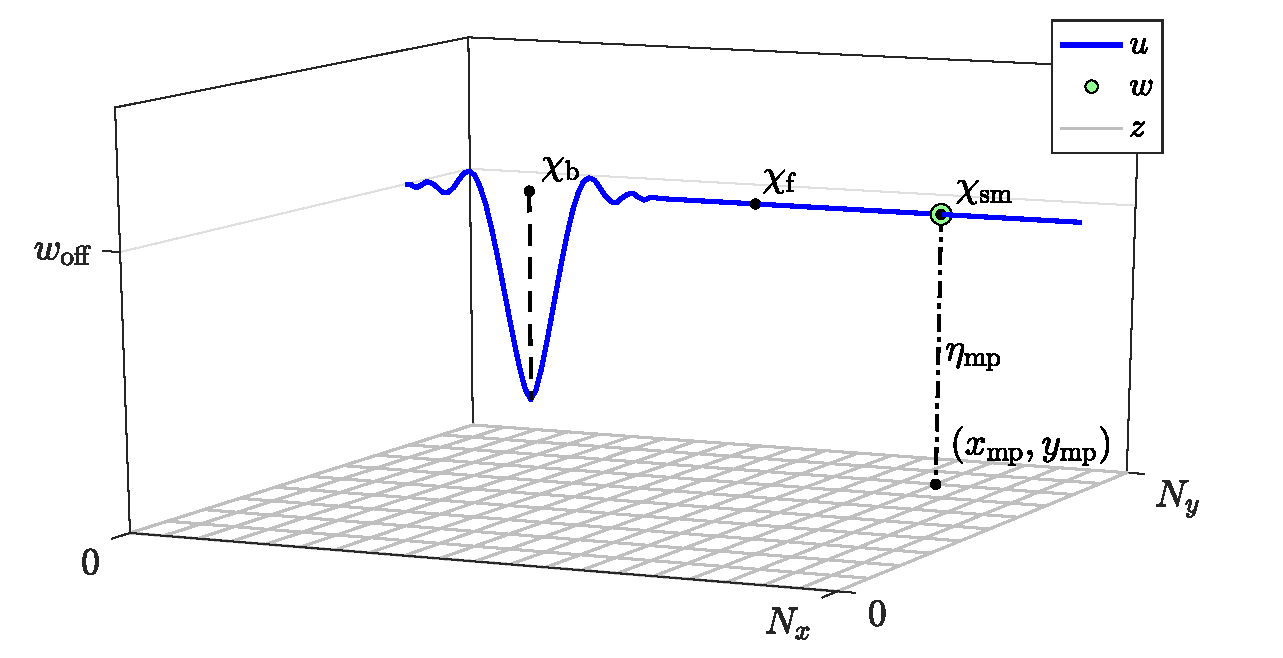
\includegraphics[width=1.0\columnwidth]{trombaSystem.eps}
  \caption{The virtual system in Equations \eqref{eq:fullSystemDisc} including the offset in Eq. \eqref{eq:offset}, with different important coordinates highlighted. Note that $\eta_\text{sm}$ (Eq. \eqref{eq:etaSMDisc}) is not shown as it is close to 0 at all times. }
  \label{fig:trombaSystem}
\end{figure}

\subsection{Pitch Control}
Secondly, as briefly mentioned in Section \ref{sec:introduction}, the way different pitches are played on the tromba marina, is to slightly rest a knuckle or finger on nodal points along the string to induce harmonics. Thus, a damping finger is implemented. Using the cubic interpolation operator $I_3$ \cite{bilbao2009numerical}, the FDS for the string in \eqref{eq:stringDisc} can be extended to
\begin{gather}\label{eq:dampingFinger}
    \ell_\text{s} u_{l,\text{s}}^n = \hdots - J_3(x_\text{f})I_3(x_\text{f})\sigma_\text{f}(u^n_l-u_\text{off}),\\
   \text{where} \quad 0\leq \sigma_\text{f} \leq 1,\nonumber
\end{gather}
which essentially subtracts its own state at location $x_\text{f} \in [0,0.5x_\text{sm}]$ according to the damping coefficient $\sigma_\text{f}$ (kg$ \cdot$ s$^{-2}$) applied. As done in \cite{Willemsen2019:SMC2020}, the fractional part used in the spreading operator ($\alpha_\text{i} = x_\text{f}/h - \text{floor}(x_\text{f}/h)$) is raised to the 7th power as it has been empirically found to scale finger position to pitch more properly in the context of FDSs. As the string is bowed above the damping finger (at the other side of the rattling bridge) it is   essential that the energy from the bow reaches the rattling bridge. For lower values for $\sigma_\text{f}$, this is still the case.

\subsection{Other Considerations}
Realistic initialisation both $\eta_\text{sm}$ and $\eta_\text{mp}$ is essential. In this case (at $n=0$) $\eta_\text{sm}^0 = 0$ and $\eta_\text{mp}^0 \leq 0$ so that no collision is present at initialisation. If this is not done, the value for the potential at the previous time step $\psi^{n-1/2}$ would not make sense \textbf{(perhaps elaborate)}.

After $h_\text{p}$ is calculated in Equation \eqref{eq:gridSpacingPlate}, we check whether it is smaller than a set value $h_{\text{p},\text{min}} = 0.01$. This reduces the quality of the model, but increases the speed, allowing for real-time implementation.

\subsection{Order of calculation} 
The order of calculation is shown in the pseudocode in Algorithm \ref{alg:calcOrder}.
\begin{algorithm}[ht]
\fbox{\parbox{0.9\linewidth}{
\setstretch{1.5}
 \While{application is running}{
 \vspace{0.15cm}
 \begin{minipage}[c]{0.48\linewidth}
1. calculate schemes\\
2. apply bow to string\\
3. apply damping finger\\
4. calculate $g^n_\text{sm}$ and $g^n_\text{mp}$\\
\vspace{-0.2cm}5. calculate collision and
\vspace{-0.2cm}connection forces and add to schemes\\
\vspace{-0.2cm}6. Update states \\
\vspace{-0.2cm}\\
\end{minipage}
\hspace{0.05cm}
\begin{minipage}[c]{0.42\linewidth}
($\ell u$ in Eqs. (\ref{eq:stringDisc}-c))\\
(Eq. \eqref{eq:stringDisc})\\
(Eq. \eqref{eq:dampingFinger})\\
(Eqs. \eqref{eq:gnSM} and \eqref{eq:gnMP})\\
\vspace{-0.2cm}(Eqs. (\ref{eq:stringDisc}-c))\\
\vspace{-0.2cm}\\
\\
\vspace{-0.2cm}$\boldsymbol{u}^{n-1} = \boldsymbol{u}^n$\\
\vspace{-0.2cm}$\boldsymbol{u}^{n} = \boldsymbol{u}^{n+1}$\\
$\boldsymbol{\psi}^{n-1/2} = \boldsymbol{\psi}^{n+1/2}$
\end{minipage}}
 }}
 \vspace{0.2cm}
 \caption{Pseudocode showing the order of calculations after initialisation.\label{alg:calcOrder}}
\end{algorithm}
%
In theory, in order to iteratively calculate the bow force, the collision and connection forces should be included in this. \SWcomment[Hmm.. but the rest of the system is explicit. Shouldn't the system be calculated in its entirety before the NR calculation?] However, as the string is practically never bowed at the bridge position $x_\text{sm}$, these can be calculated independently.

\subsection{Parameter design}
The list of parameters used can be found in Table \ref{tab:parameters}. As the authors had a real (recreated) tromba marina (presented in \cite{Baldwin2016:SMC2020}) at their disposal, some parameters have been measured in accordance to the real instrument.

Regarding the output of the system, through empirical testing it was decided to retrieve the output from the state of the plate right at the point of collision $(x_\text{mp},y_\text{mp})$ combined with the sound of the string at a lower volume. It can be argued that the loudest sound comes from the collision between the bridge and the body making it logical to select this point as the output position. 

\begin{table}[t]\label{tab:parameters}
\small
\begin{center}
\begin{tabular}{|l|c|c|}
    \hline
    Name & Symbol (unit) & Value\\ \hline
    \multicolumn{3}{|l|}{\bf String}\\ \hline
    Length & $L$ (m) & $1.90$*\\
    Material density & $\rho_\text{s}$ (kg$\cdot$m$^{-3}$) & $7850$\\ 
    Radius & $r$ (m) & $0.0005$\\
    Fundamental freq. & $f_0$ (s$^{-1}$)& $32.0$*\\ 
    Young's modulus & $E_\text{s}$ (Pa) & $2\cdot 10^{11}$\\
    Freq. indep. loss & $\sigma_{0,\text{s}}$ (s$^{-1}$) & $0.1$\\ 
    Freq. dep. loss & $\sigma_{1,\text{s}}$ (m$^2$/s) & $0.05$\\ \hline
    \multicolumn{3}{|l|}{\bf Bow}\\ \hline
    Bow force & $F_\text{b}$ (N) & $0 \leq F_\text{b} \leq 0.1 $\\
    Bow velocity & $v_\text{b}$ (m/s) & $-0.5 \leq v_\text{b} \leq 0.5 $\\
    Free parameter & $a$ (-) & $100$\\\hline
    \multicolumn{3}{|l|}{\bf Bridge}\\ \hline
    Mass & $M$ (kg) & $0.001$\\ 
    Fundamental freq. & $f_{0,\text{m}}$ (s$^{-1}$) & $500$\\ 
    Damping & $R$ (s$^{-1}$)& $0.05$\\
    \hline
    \multicolumn{3}{|l|}{\bf Body}\\ \hline
    Length & $L_x$ (m)& $1.35$*\\ 
    Width & $L_y$ (m)& $0.18$*\\ 
    Material density & $\rho_\text{p}$ (kg$\cdot$m$^{-3}$)& $50$\\ 
    Thickness (m) & $H$ (m) & $0.01$\\ 
    Young's modulus & $E_\text{p}$ (Pa) & $2\cdot 10^{5}$\\ 
    Poisson's ratio & $\nu$ (-)& $0.3$\\
    Freq. indep. loss & $\sigma_{0,\text{p}}$ (s$^{-1}$)& $2$\\
    Freq. dep. loss & $\sigma_{1,\text{p}}$ (m$^2$/s)& $0.05$\\ \hline
    \multicolumn{3}{|l|}{\bf String-bridge connection}\\\hline
    Stiffness Coefficient & $K_\text{sm}$ (N/m) & $5\cdot10^{6}$\\
    Non-lin. col. coeff. &$\alpha_\text{sm}$ (-) & 1.0\\
    Bridge location & $x_\text{sm}$ (m)& $1.65$*\\
    \hline
    \multicolumn{3}{|l|}{\bf Bridge-body collision}\\\hline
    Stiffness Coefficient & $K_\text{mp}$ (N/m) & $5\cdot10^{8}$\\
    Non-lin. col. coeff. &$\alpha_\text{mp}$ (-) & 1.0\\
    Bridge location & ($x_\text{mp},y_\text{mp}$) (m,m)& $(1.08,0.135)$*\\\hline
    \multicolumn{3}{|l|}{\bf Other}\\\hline
    Offset & $u_\text{off}$ (m) & $5\cdot 10^{-6}$\\
    Damp. finger coeff. &$\sigma_\text{f}$ (kg$\cdot$s$^{-2}$)&$0\leq \sigma_\text{f} \leq 1$\\
    \hline
\end{tabular}
\caption{List of parameter values used for the simulation. *These values have been taken from a real (recreated) tromba marina \cite{Baldwin2016:SMC2020}.}
\end{center}
\end{table}

\subsection{Graphical User Interface}\label{sec:GUI}
A screenshot of the GUI is shown in Figure \ref{fig:GUI}. The GUI is divided in four sections, three showing the states of the string, bridge and body respectively and one control section. 

 Firstly, the string section shows the state of the string $u_{l,\text{s}}^n$ as a cyan-coloured path and the bow as a yellow rectangle with bow position $x_\text{b}$ and its opacity depending on the bow force $F_\text{b}$. Furthermore, the bridge state $u_\text{m}^n$ is shown as a green circle at location (of the bridge along the string) $x_\text{sm}$. Finally, the position of the damping finger $x_\text{f}$ is displayed as a yellow circle, the size of which depends on damping coefficient $\sigma_\text{f}$. The position of the finger triggers lines showing the locations of the closest nodes along the string according to the following equation
\begin{equation}
    x_\text{node}^i = \frac{i\cdot x_\text{sm}}{n}\quad \text{for} \quad i = [1,\hdots,n-1],
\end{equation}
where $n = \text{round} (x_\text{sm}/x_\text{f})$ is an integer closest to the ratio between the string length until the bridge location and the damping finger position. These lines are drawn is to help the user place the damping finger at nodes along the string.

Secondly, the bridge section shows the displacement of the bridge $u_\text{m}^n$ as a green circle, the state of the body at the collision location $u_{(x_\text{sm},y_\text{sm}),\text{p}}^n$, both moving vertically with their respective displacements and finally, a grey horizontal line denoting the offset $u_\text{off}$, i.e., the resting position of the bridge.

Thirdly, the body section shows the state of the body as a grid of rectangles changing (grey-scale) colour with displacement (white for positive and black for negative).


Finally, the control section contains three sliders that control the levels of the string (s), bridge (m) and body (p) respectively and a reset button to re-initialise the system. 
\begin{figure}[h]
  \centering
  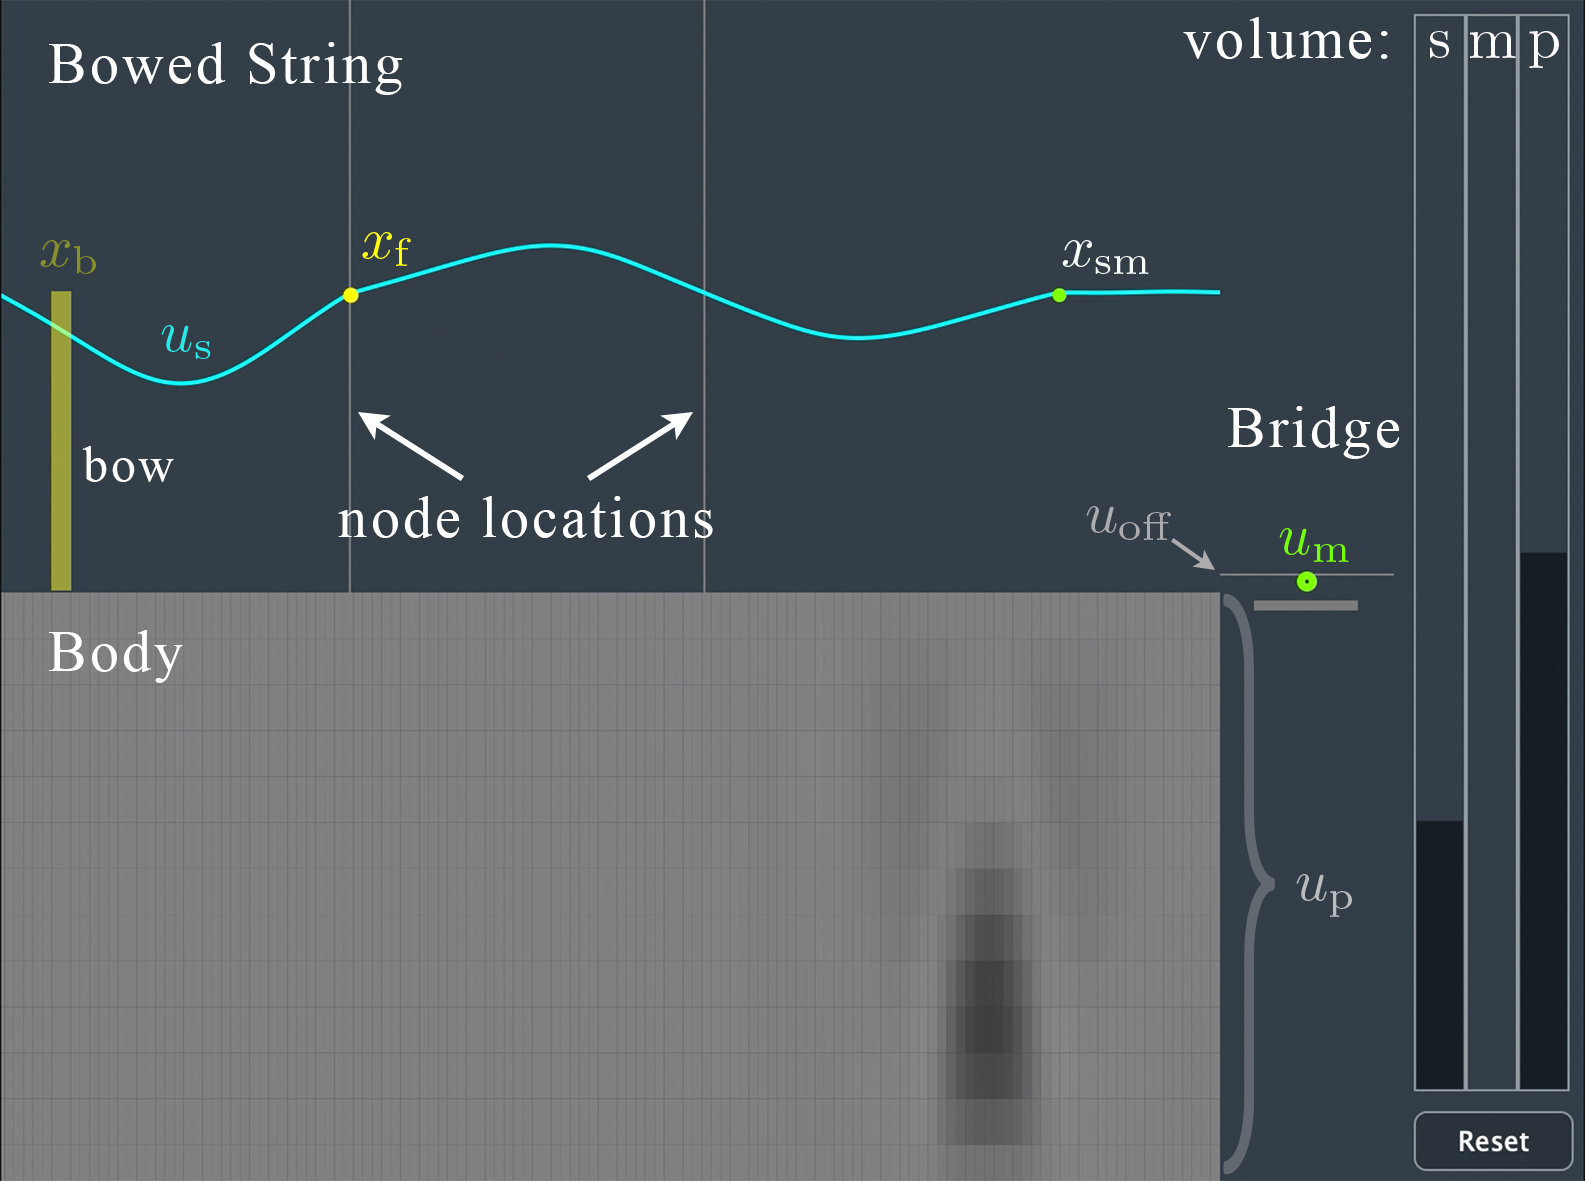
\includegraphics[width=1.0\columnwidth]{applicationDescription.png}
  \caption{The GUI showing the excited system with text highlighting different components. A detailed description of this figure can be found in Section \ref{sec:GUI}.}
  \label{fig:GUI}
\end{figure}

\subsection{Sensel Morph and Mapping}
The Sensel is an expressive touch controller using \texttildelow20,000 pressure sensitive sensors laid out in an hexagonal grid\cite{sensel2020}. It retrieves x and y positions and pressure at a rate of 150 Hz from which velocities and accelerations can be obtained.

The first finger registered by the Sensel is mapped to the bow: x-position is mapped to bow position $x_\text{b}$, y-velocity to bow velocity $v_\text{b}$ (y-position is shown in the GUI but does not influence the model directly) and pressure to bow force $F_\text{b}$. The second finger is mapped to the damping finger: x-position is mapped to finger location $x_\text{f}$ and pressure to damping coefficient $\sigma_\text{f}$.

\section{Discussion}

As can be seen from Table \ref{tab:parameters}, the non-linear collision coefficients $\alpha_\text{sm}$ and $\alpha_\text{mp}$ are set to $1$. We found some odd behaviour when increasing this value, where the bridge would `get stuck' behind the plate, i.e., values for $\psi_\text{mp}$ would be negative for a prolonged period of time. The explicit technique used in this work allows for this to happen (and can be proven to still be stable in this case \cite{Ducceschi2019}), but it is unphysical to have a negative potential. Futher investigation will be necessary to figure out a way to prevent this behaviour.

\section{Conclusions}
Comparison between NR and Non-iterative methods (both speed and quality)

Parameter design

For a more physical implementation of the damping finger, it might be a good idea to model it as another mass colliding with the string rather than imposing a `hacky' way of damping onto the string state. 
\begin{acknowledgments}
This work is supported by NordForsk's Nordic
University Hub Nordic Sound and Music Computing Network
NordicSMC, project number 86892. Ducceschi's work was supported by an Early Career Fellowship from the Leverhulme Trust.
\end{acknowledgments} 

%%%%%%%%%%%%%%%%%%%%%%%%%%%%%%%%%%%%%%%%%%%%%%%%%%%%%%%%%%%%%%%%%%%%%%%%%%%%%
%bibliography here
{\small
\bibliography{smc2020bib}
}
\end{document}
